\begin{frame}
    \frametitle{Aufgabe 5}
    \framesubtitle{}
    \begin{itemize}
        \item Untersuchung des Signalverhaltens bei Koaxialkabeln
    \end{itemize}
\end{frame}
\begin{frame}
    \frametitle{Aufgabe 5}
    \framesubtitle{Signalgeschwindigkeit}
    \begin{itemize}
        \item Kabelende wird offen gelassen
        \item Beobachtung: Zwei Pulse hintereinander durch Signalreflexion am
        offenen Kabelende
    \end{itemize}
    \begin{figure}[H]
    \begin{center}
            \includegraphics[scale=0.2]{./img/5a.png}
    \end{center}
    \end{figure}
\end{frame}
\begin{frame}
    \frametitle{Aufgabe 5}
    \framesubtitle{Signalgeschwindigkeit}
    \begin{itemize}
        \item Signal wird am offenen Kabelende reflektiert
        \item Signalgeschwindigkeit: $ v = \frac{20m}{100ns}=2 \cdot 10^8
        ms^{-1}$
    \end{itemize}
\end{frame}
\begin{frame}
    \frametitle{Aufgabe 5}
    \framesubtitle{Abschlusswiderstand}
    \begin{itemize}
        \item Kabelende wird mit Potentiometer abgeschlossen
        \item Widerstand wird variiert
    \end{itemize}
    \begin{figure}[H]
    \begin{center}
            \includegraphics[scale=0.2]{./img/5b_Potentiometer_1.png}
    \end{center}
    \end{figure}
\end{frame}
\begin{frame}
    \frametitle{Aufgabe 5}
    \framesubtitle{Abschlusswiderstand}
    \begin{itemize}
        \item Kabelende wird mit Potentiometer abgeschlossen
        \item Widerstand wird variiert
    \end{itemize}
    \begin{figure}[H]
    \begin{center}
            \includegraphics[scale=0.2]{./img/5b_Potentiometer_3.png}
    \end{center}
    \end{figure}
\end{frame}
\begin{frame}
    \frametitle{Aufgabe 5}
    \framesubtitle{Abschlusswiderstand}
    \begin{itemize}
        \item Kabelende wird mit Potentiometer abgeschlossen
        \item Widerstand wird variiert
    \end{itemize}
    \begin{figure}[H]
    \begin{center}
            \includegraphics[scale=0.2]{./img/5b_Potentiometer_2.png}
    \end{center}
    \end{figure}
    \begin{itemize}
        \item Auslöschung des Signals bei $R=53.62 \Omega$
    \end{itemize}
\end{frame}
\begin{frame}
    \frametitle{Aufgabe 5}
    \framesubtitle{Abschlusswiderstand}
    \begin{itemize}
        \item Kabel wird mit $50 \Omega$ abgeschlossen $\rightarrow$
        Auslöschung des Signals
    \end{itemize}
    \begin{figure}[H]
    \begin{center}
            \includegraphics[scale=0.2]{./img/5b_Abschluss.png}
    \end{center}
    \end{figure}
\end{frame}
\begin{frame}
    \frametitle{Aufgabe 5}
    \framesubtitle{Abschlusswiderstand}
    \begin{itemize}
        \item Abschlusswiderstand kann Signal abdämpfen und auslöschen
        \item längere Impulssignale können sich überlagern 
    \end{itemize}
    \begin{center}
    \begin{tabular}{c|c c}
    & Messwerte & Datenblatt \\
    \hline
    v & $2 \cdot 10^{8} ms^{-1}$ & $2 \cdot 10^{8} ms^{-1}$ \\
    C'& $93.249 pFm^{-1}$&$100.7 pFm^{-1}$ \\
    L'& $268.1 nHm^{-1}$& keine Angabe \\
    R & $53.62 \Omega$& $50 \Omega$
    \end{tabular}
    \end{center}
\end{frame}
\begin{frame}
    \frametitle{Aufgabe 5}
    \framesubtitle{Einfache Laufzeit}
    \begin{itemize}
        \item Kabel wird an Kanal des Oszilloskops angeschlossen
    \end{itemize}
    \begin{figure}[H]
    \begin{center}
            \includegraphics[scale=0.2]{./img/5c_zweiter_Kanal.png}
    \end{center}
    \end{figure}
\end{frame}
\begin{frame}
    \frametitle{Aufgabe 5}
    \framesubtitle{Einfache Laufzeit}
    \begin{figure}[H]
    \begin{center}
            \includegraphics[scale=0.2]{./img/5c_zweiter_Kanal.png}
    \end{center}
    \end{figure}
    \begin{itemize}
        \item Erklärung:
        \begin{itemize}
            \item Kabel kommt an Kanal 1 an (gelb)
            \item Kabel kommt an Kanal 2 an (grün)
            \item Kabel wird an Kanal 2 reflektiert und wird in Kanal 1 (gelb)
            gemessen
        \end{itemize}
    \end{itemize}
\end{frame}
\begin{frame}
    \frametitle{Aufgabe 5}
    \framesubtitle{Einfache Laufzeit}
    \begin{itemize}
        \item Kanal 2 wird mit Abschlusswiderstand abgeschlossen
    \end{itemize}
    \begin{figure}[H]
    \begin{center}
            \includegraphics[scale=0.2]{./img/5c_zweiterKanal_Abschlusswiserstand_1.png}
    \end{center}
    \begin{itemize}
        \item Abschlusswiderstand löscht Signal aus $\rightarrow$ keine
        Reflexion
    \end{itemize}
    \end{figure}
\end{frame}
\begin{frame}
    \frametitle{Aufgabe 5}
    \framesubtitle{Dämpfung}
    \begin{itemize}
        \item $100m$ Kabel wird mit Sinusspannung untersucht
    \end{itemize}
\end{frame}
\begin{frame}
    \frametitle{Aufgabe 5}
    \framesubtitle{Dämpfung}
    \begin{figure}[H]
    \begin{center}
            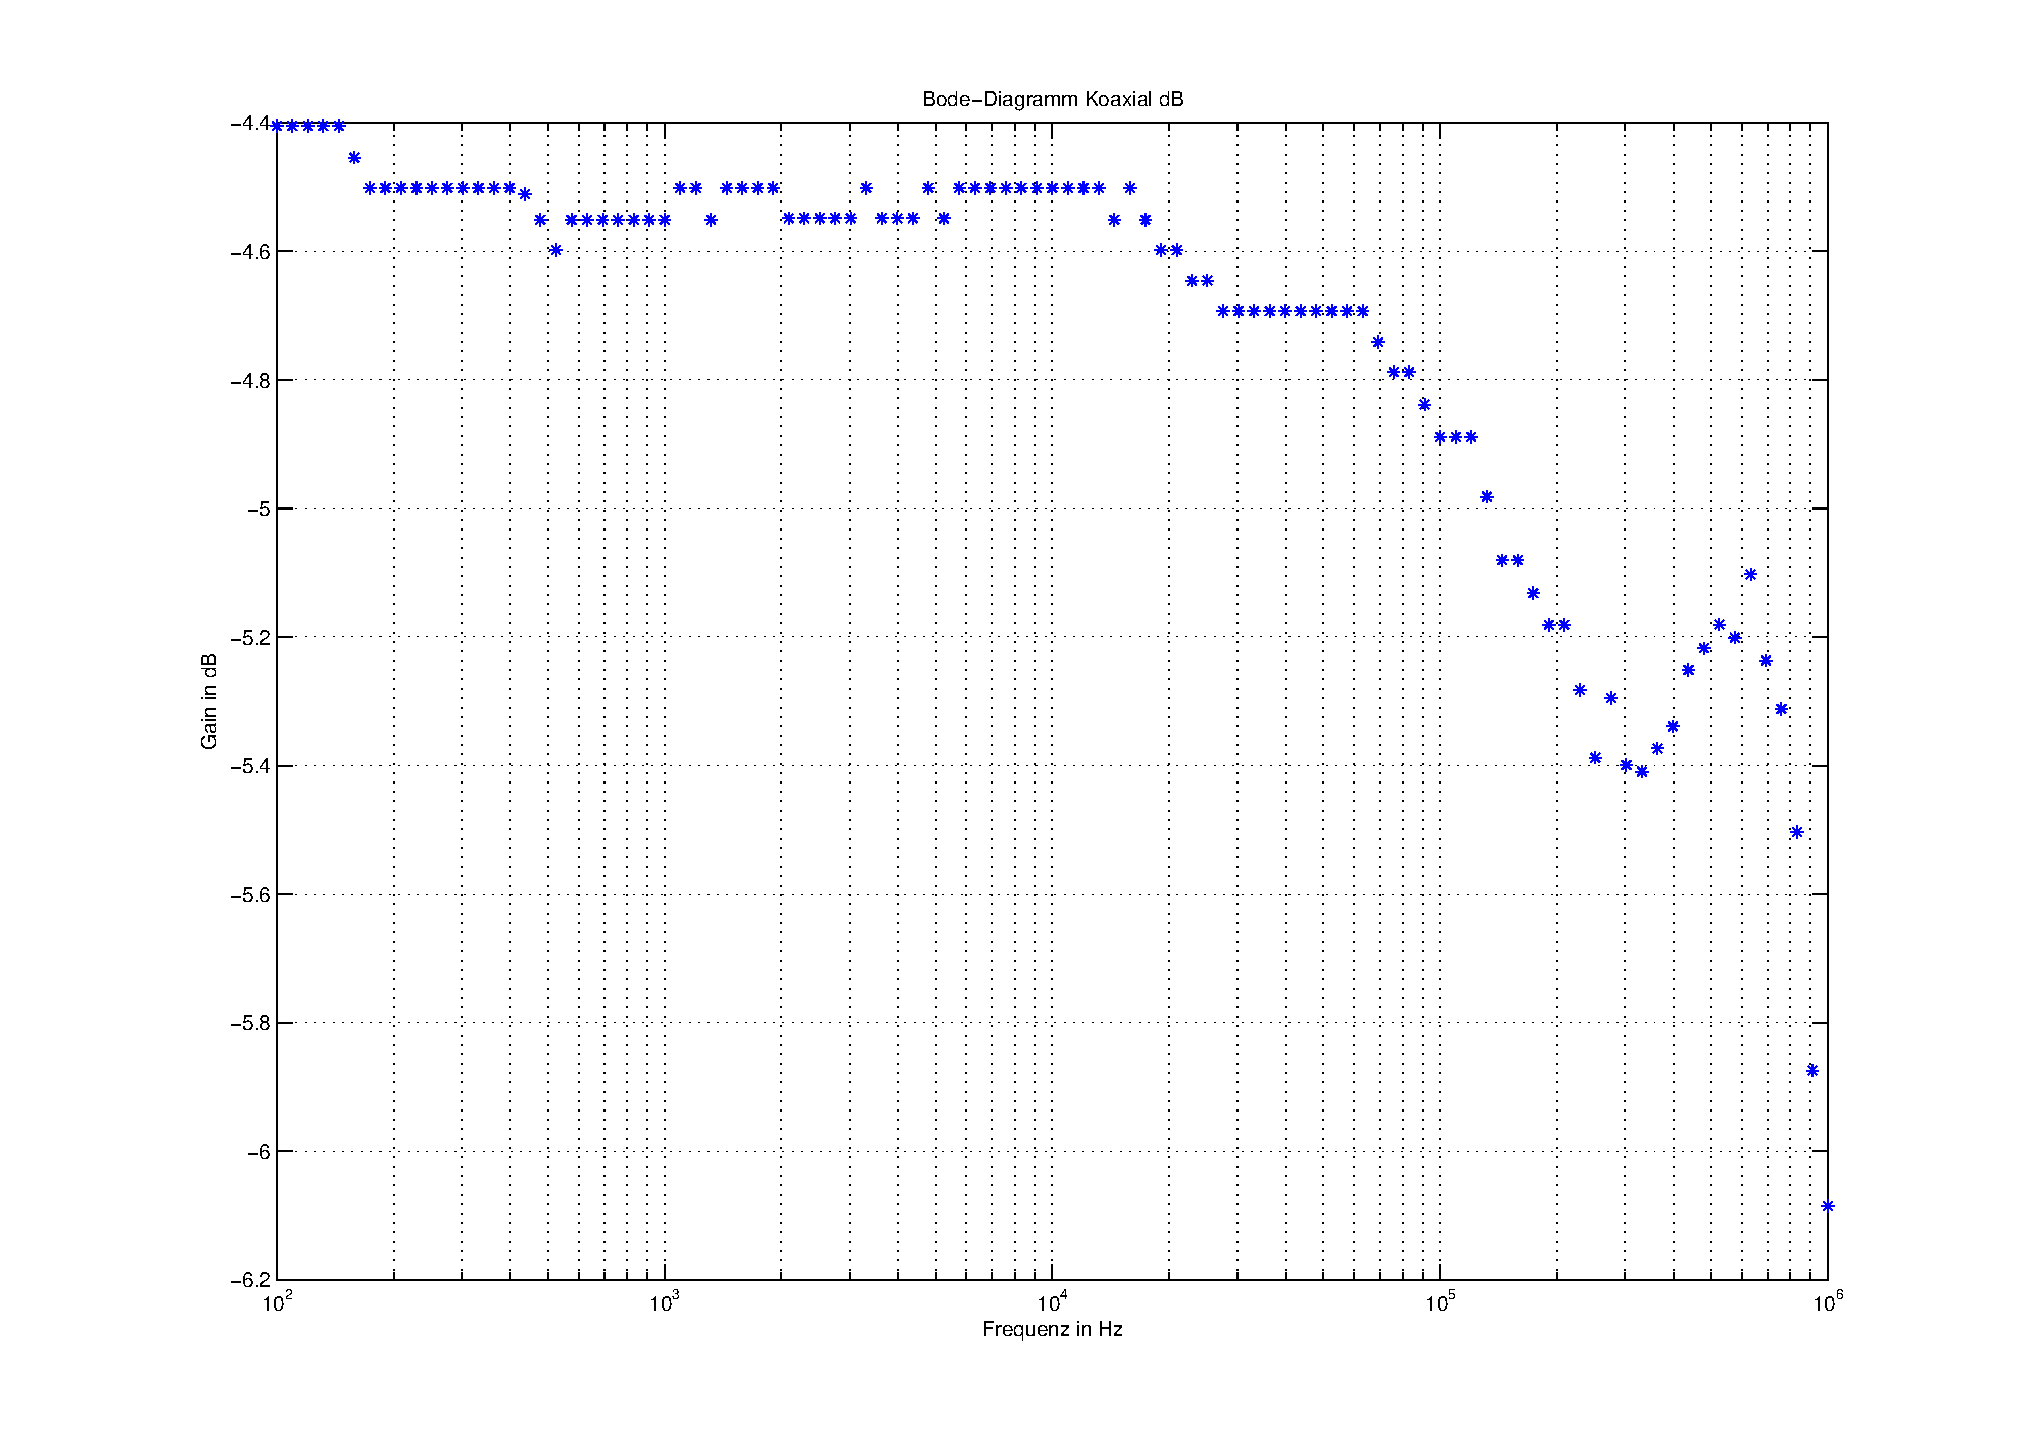
\includegraphics[scale=0.6]{./img/5d_bode_dB.eps}
    \end{center}
    \end{figure}
\end{frame}
\begin{frame}
    \frametitle{Aufgabe 5}
    \framesubtitle{Dämpfung}
    \begin{figure}[H]
    \begin{center}
            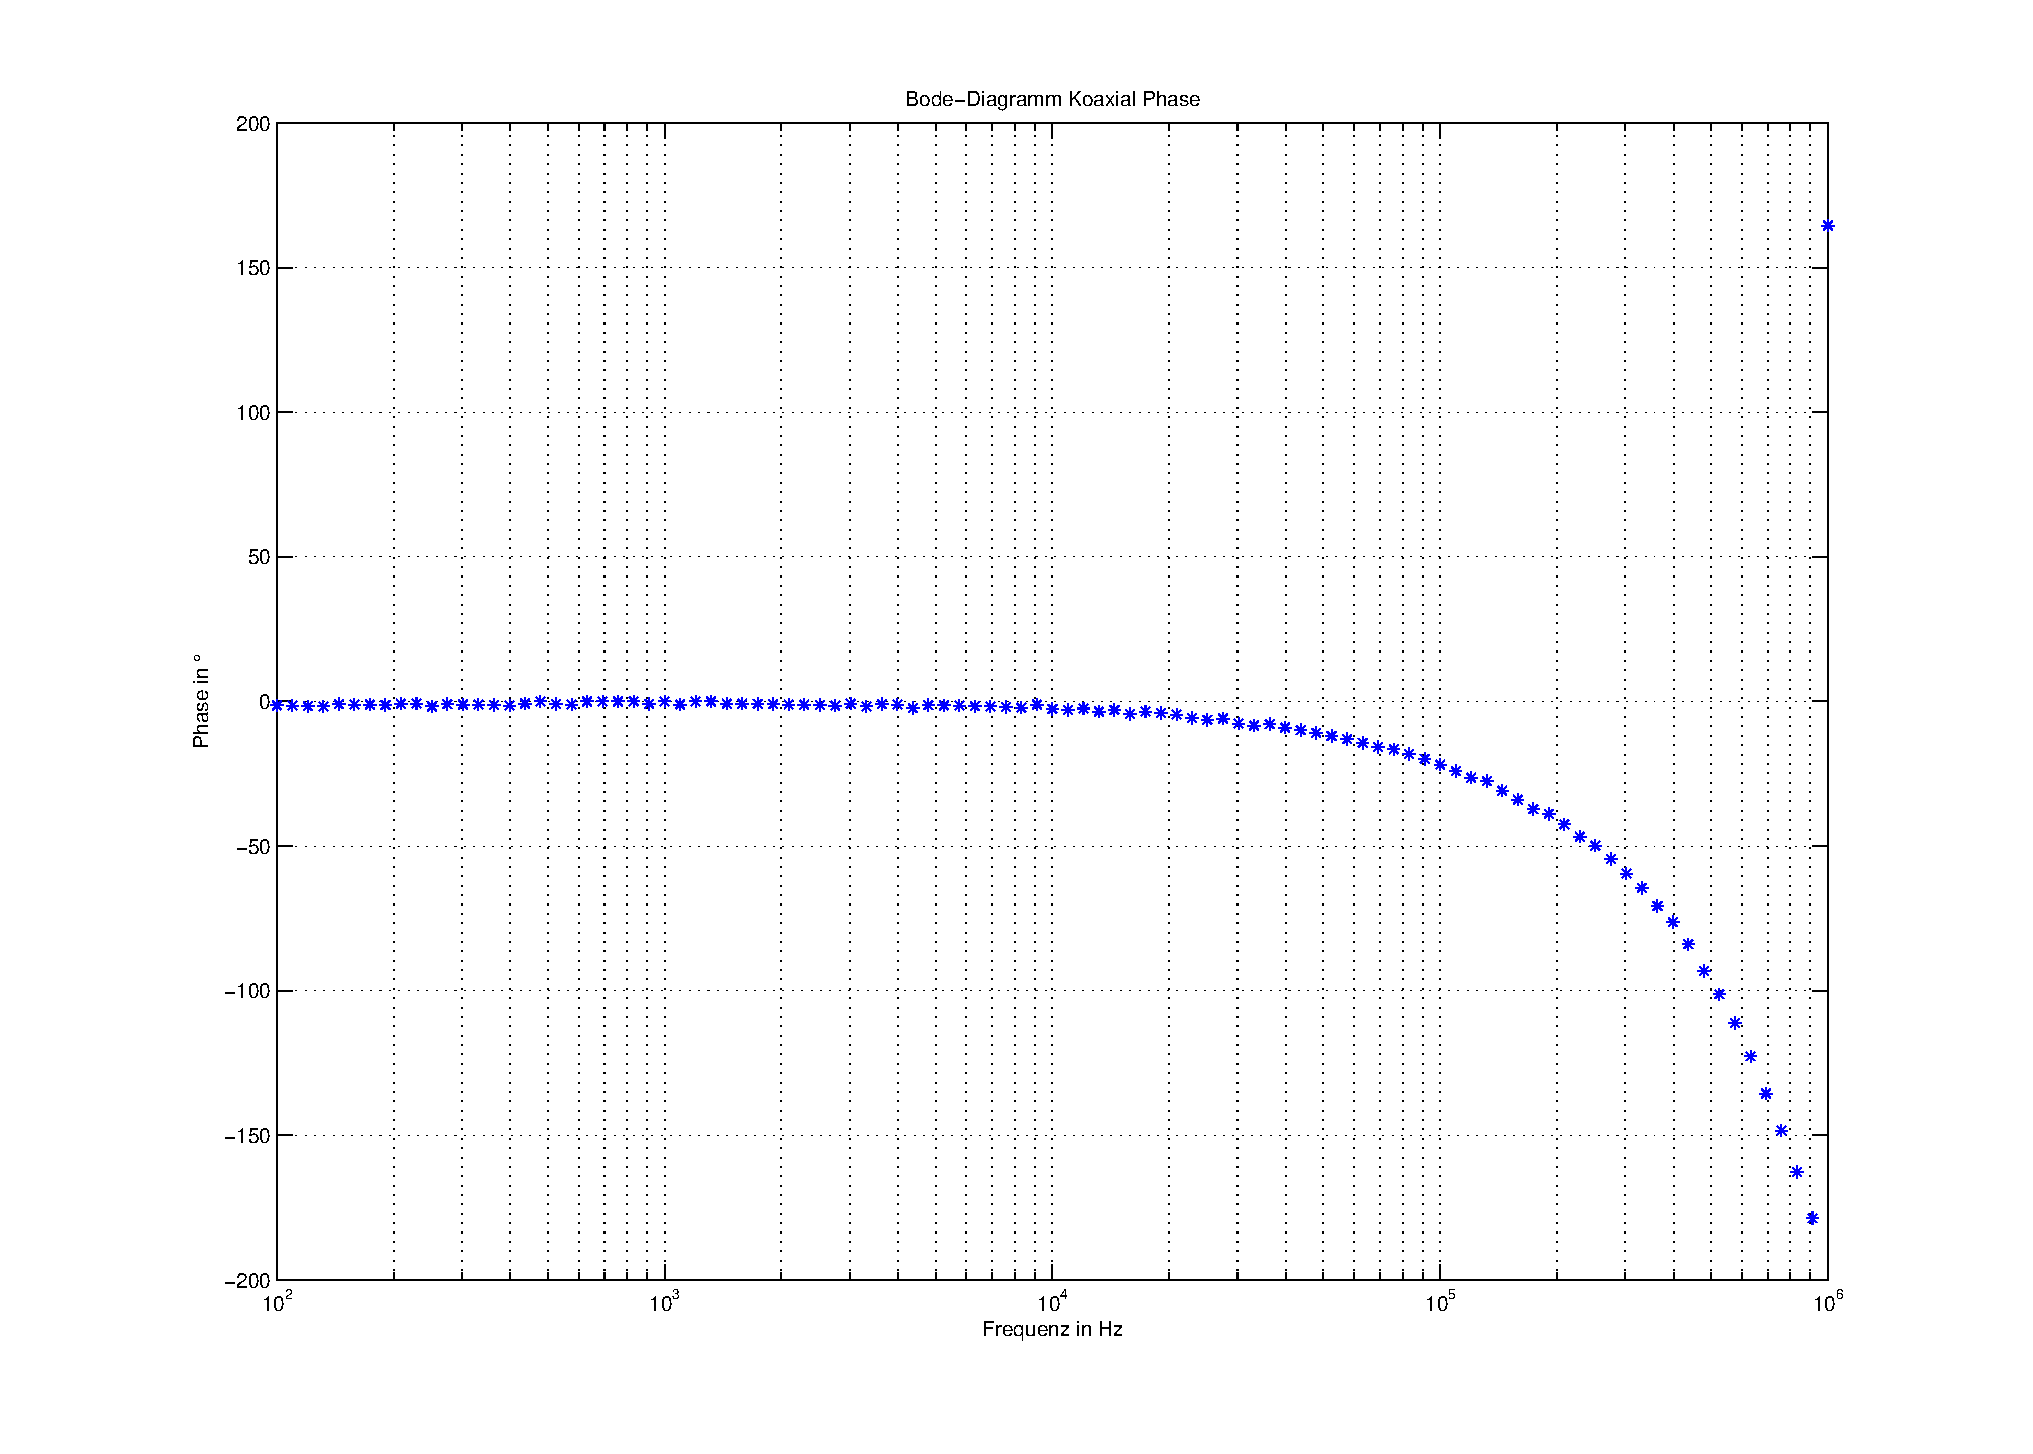
\includegraphics[scale=0.6]{./img/5d_bode_phase.eps}
    \end{center}
    \end{figure}
\end{frame}
\begin{frame}
    \frametitle{Aufgabe 5}
    \framesubtitle{Dämpfung}
    \begin{itemize}
        \item Kabel wirkt wie Tiefpassfilter
        \item Phase oszilliert stark ab $10^6 Hz$
    \end{itemize}
\end{frame}
